\documentclass[12pt]{article}
\usepackage{amsmath,amssymb,latexsym}
\usepackage{graphicx,psfrag,epsf}
\usepackage{enumerate}
\usepackage{natbib}
\usepackage{wrapfig}

\newcommand{\blind}{0}

\addtolength{\oddsidemargin}{-.75in}%
\addtolength{\evensidemargin}{-.75in}%
\addtolength{\textwidth}{1.5in}%
\addtolength{\textheight}{1.3in}%
\addtolength{\topmargin}{-.8in}%
\pagenumbering{gobble}

\begin{document}
\pagenumbering{arabic}

%\bibliographystyle{natbib}

\def\spacingset#1{\renewcommand{\baselinestretch}%
{#1}\small\normalsize} \spacingset{1}


%%%%%%%%%%%%%%%%%%%%%%%%%%%%%%%%%%%%%%%%%%%%%%%%%%%%%%%%%%%%%%%%%%%%%%%%%%%%%%

\if0\blind
{
  \title{\bf The Explanation for The Migical Phenomenon of The Rainbow Ring}
  \author{Stanley Zheng}
  \maketitle
} \fi

\if1\blind
{
  \bigskip
  \bigskip
  \bigskip
  \begin{center}
    {\LARGE\bf Title}
\end{center}
  \medskip
} \fi

\bigskip
\begin{abstract}
The stationary vertical hanging rainbow circle, after the upper end is released, will show a different phenomenon from the free fall of ordinary objects, its bottom end remains suspended in the air, and the upper end shrinks down in turn to the low end, collapses to the minimum length before starting to do the overall falling motion. Aiming to explain the interesting phenomenon of rainbow circle falling, a physical model is established, and the dynamic principle we have learned is used for detailed quantitative analysis.
\end{abstract}


\spacingset{1.45}
\section*{Introduction}
\label{sec:intro}

The rainbow ring is a very interesting coil spring toy that can be only extended, which means it is a kind of tension spring. It have many magical characteristics, and a skilled performer can use it to achieve impressive actions. Therefore, it has been welcomed and loved by everyone since its launch. There is an interesting phenomenon when the rainbow circle falls: lift the upper end of the rainbow circle, first let it be in a stationary hanging state, and it is stretched under the action of its own gravity. When the upper end is released from rest, the falling process of the rainbow circle is shown in Figure 1. Its movement is different from the general falling motion. It falls from top to bottom, until it downs to the lowest point, collapses into a closely arranged whole item and then begins to do falling motion downward. Before the rainbow ring shrinks into a whole, its bottom end is suspended in the air for a period of time as if it is magical, and only then begins to do the overall downward falling motion until it completely collapses. This amazing phenomenon has attracted many curious people, and a large number of videos of the falling process of rainbow circles can be seen on the Internet. How to explain the wonderful phenomenon of the rainbow circle? In this paper, I will establish physical models, conduct detailed quantitative analysis, and then give a reasonable physical explanation.

\begin{figure}[h]
\hspace*{1.5cm}
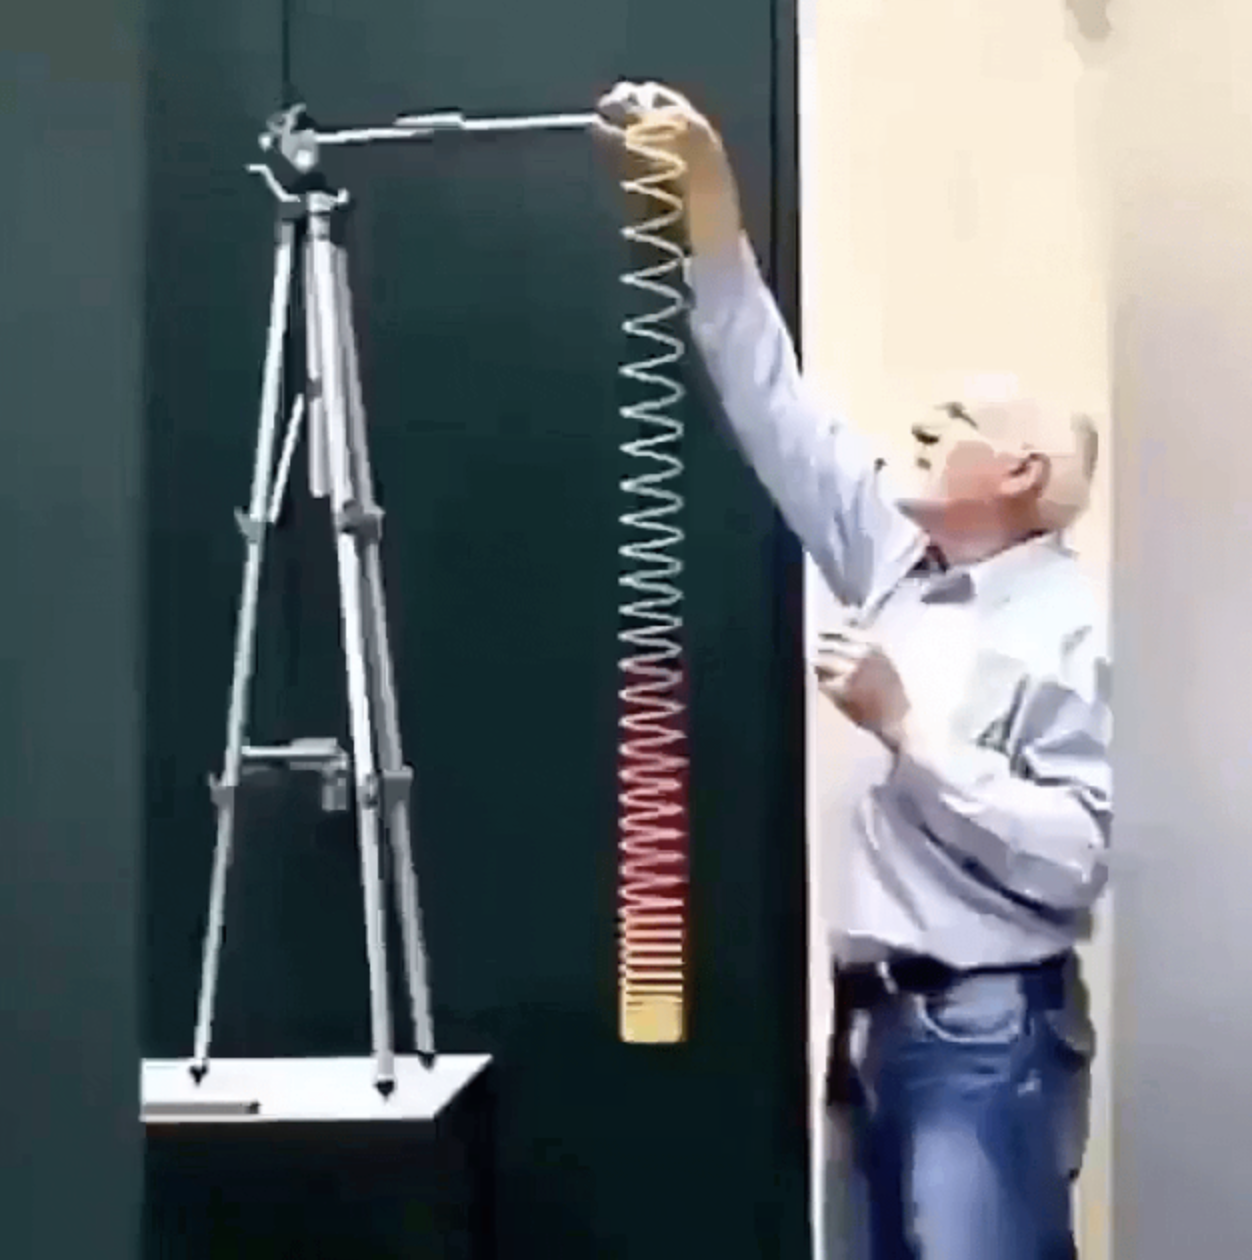
\includegraphics[width=0.2\linewidth]{1.png}
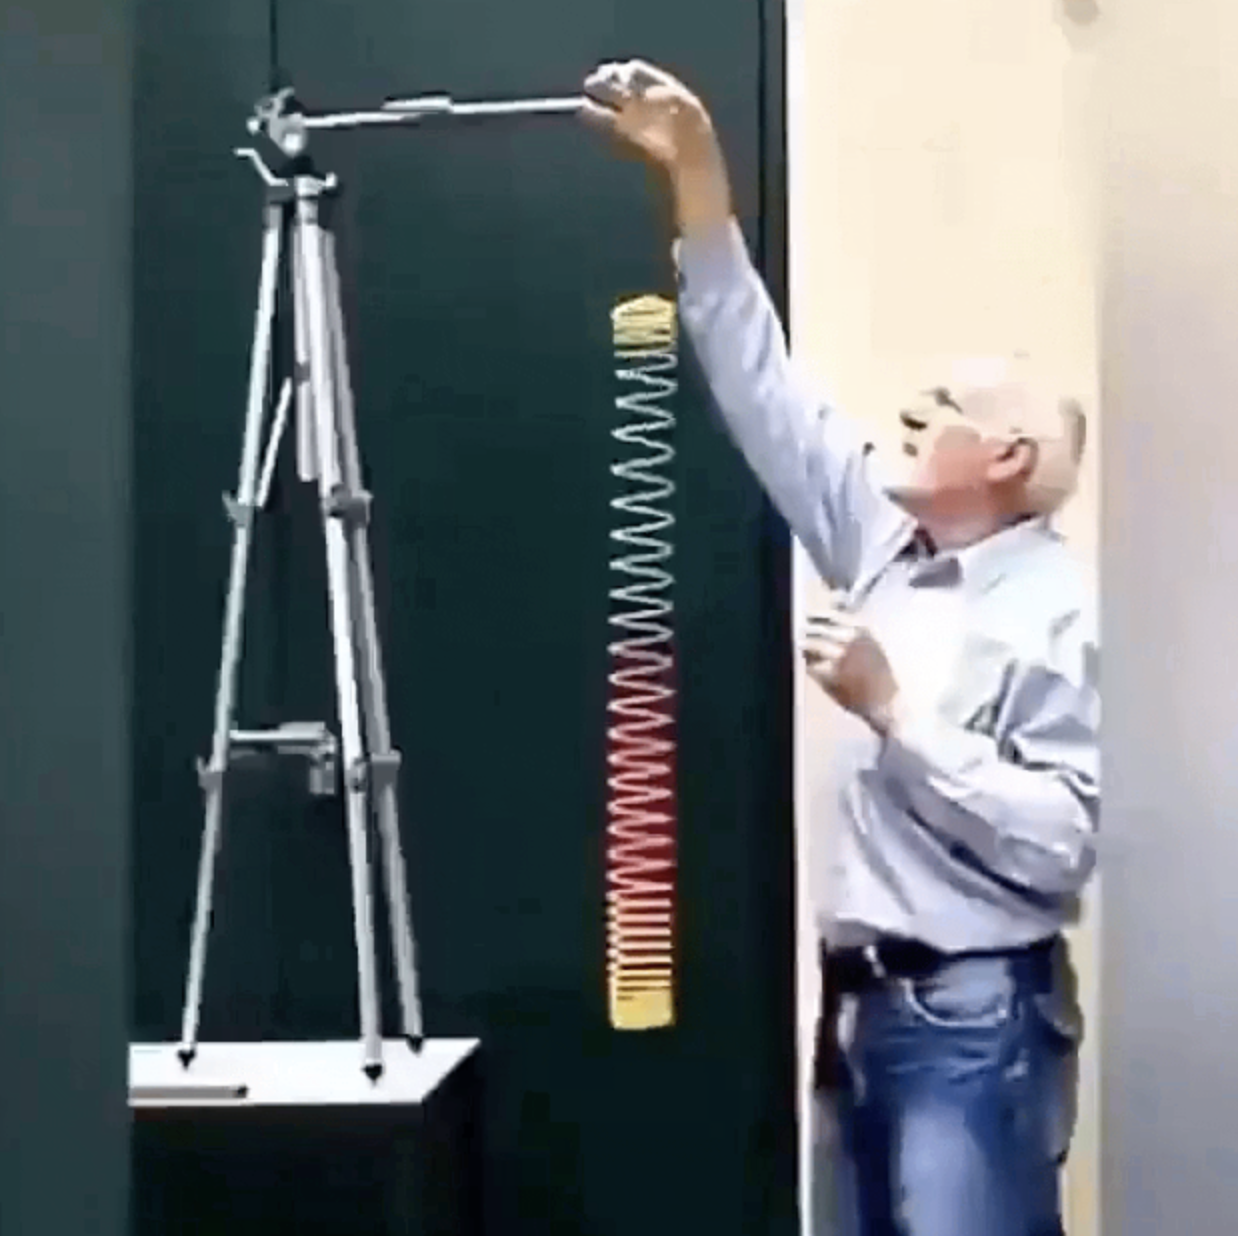
\includegraphics[width=0.2\linewidth]{2.png}
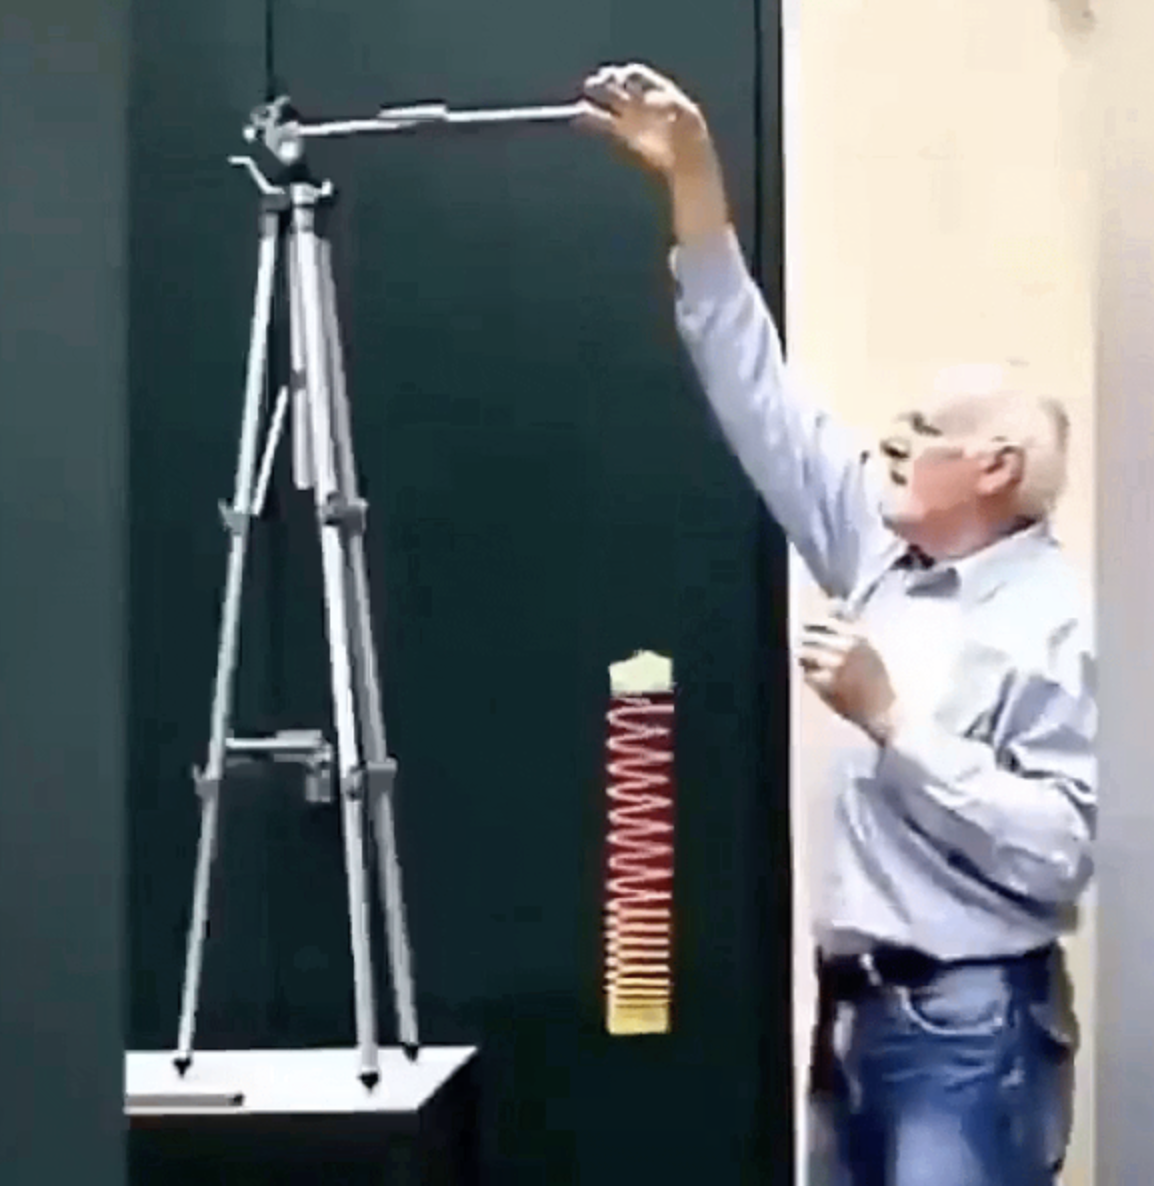
\includegraphics[width=0.2\linewidth]{3.png}
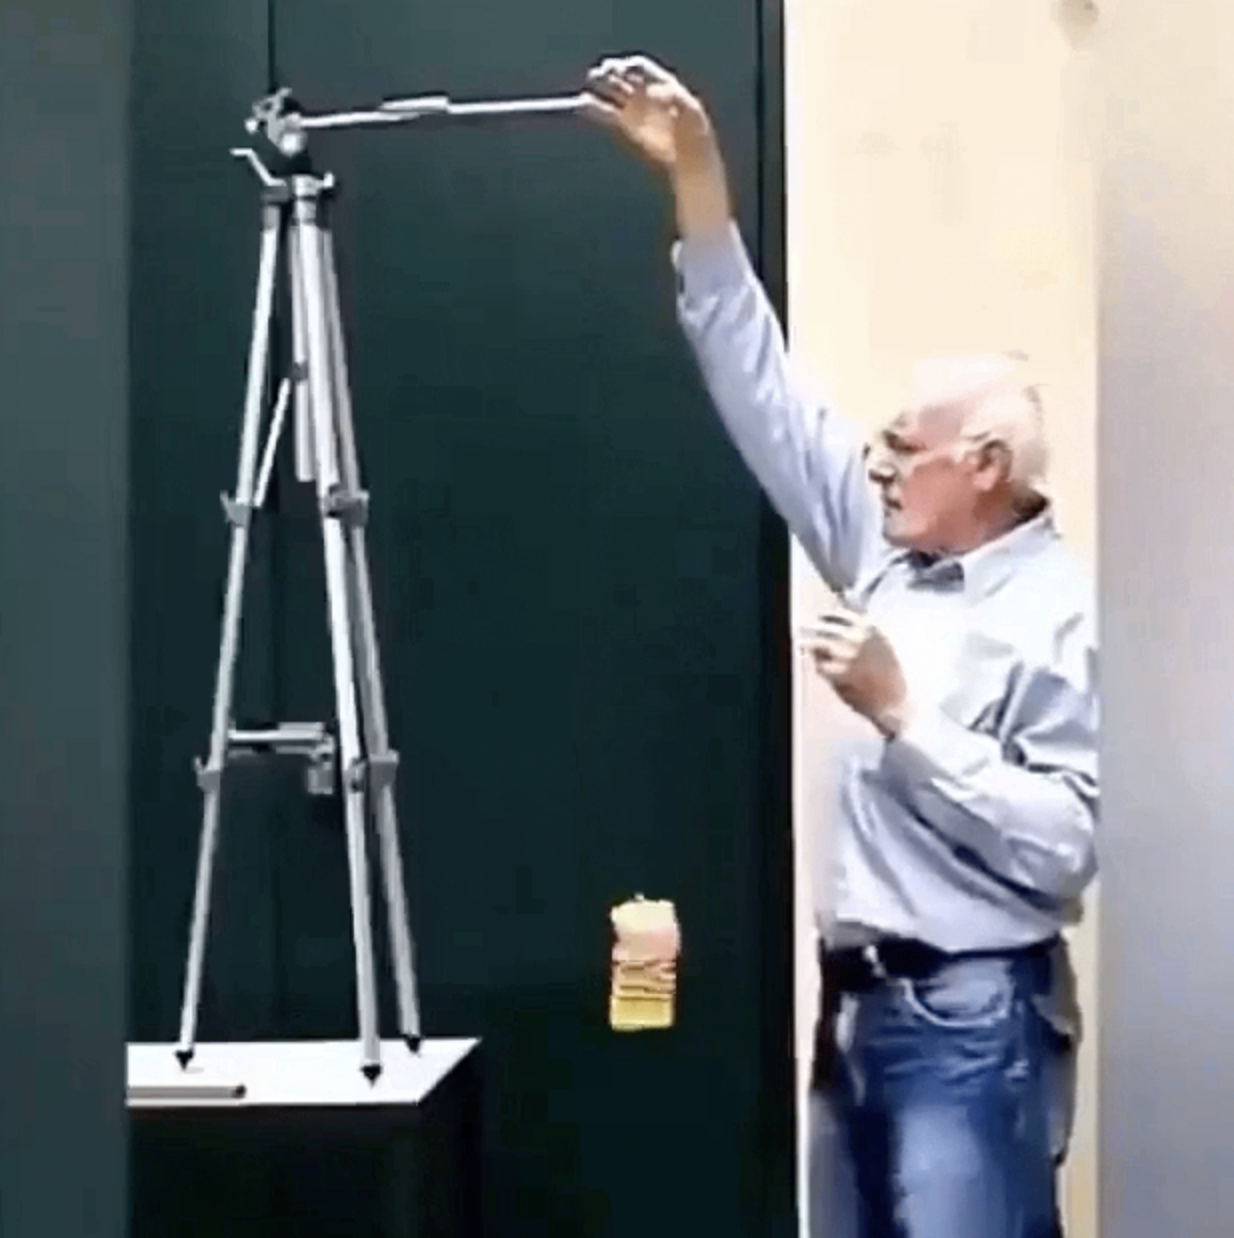
\includegraphics[width=0.2\linewidth]{4.png}
\caption{The falling movement of the rainbow ring.}
\end{figure}


\section*{Before Falling}
\label{sec:Befor}
Assuming the original length of the rainbow ring is $l_0$, the mass of the rainbow ring is $m$, the gravity is $g$, the stiffness coefficient of the rainbow ring is $k$.

Then, making the ground as the reference frame, build the 1-dimension coordinate system as the Figure 2 shows. 

\begin{figure}[h]
    \centering
    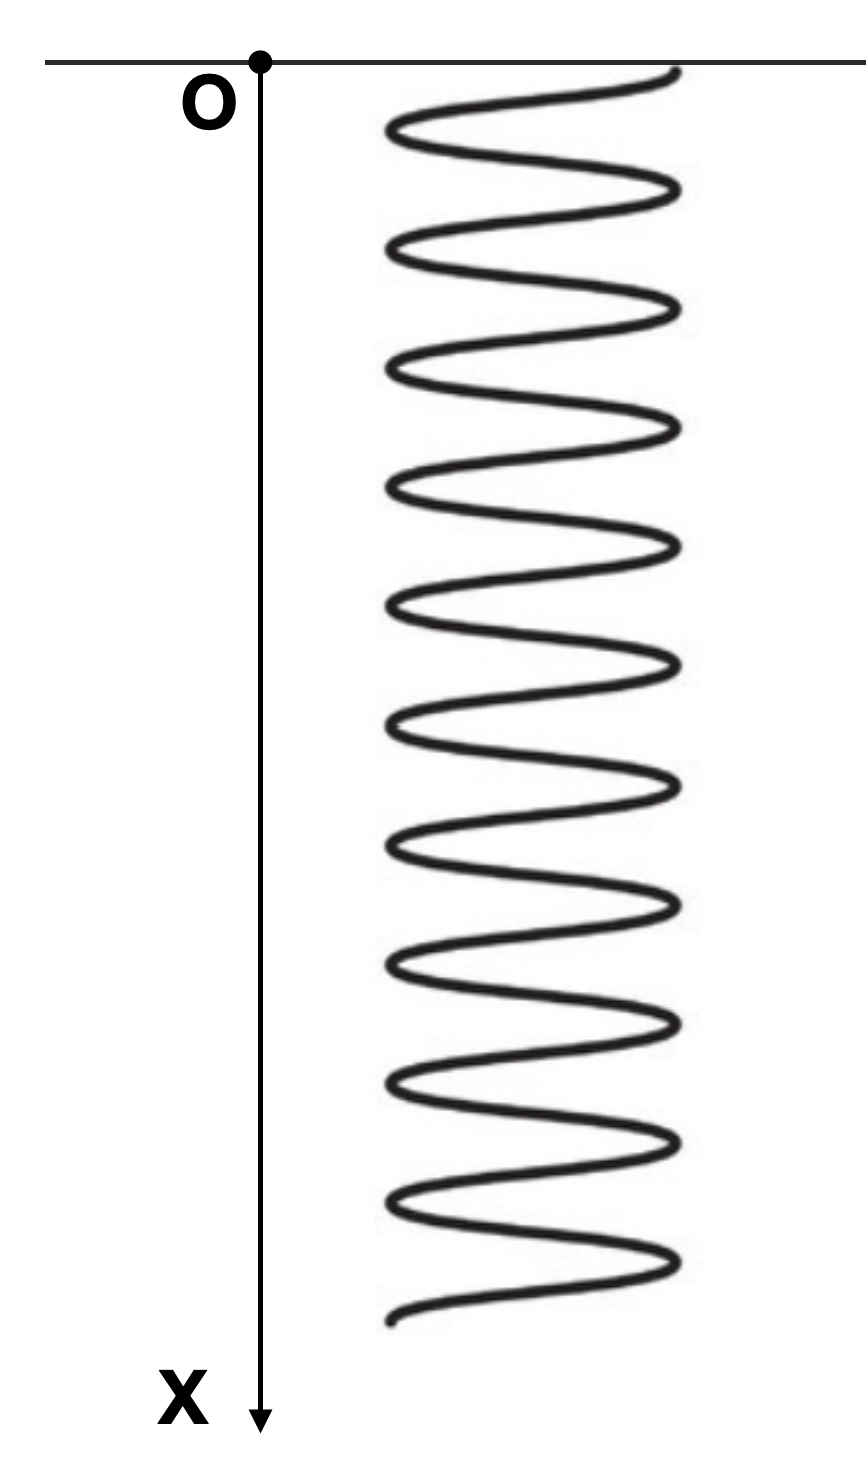
\includegraphics[width=0.2\linewidth]{5.png}
    \caption{The coordinate system.}
\end{figure}

We want to get the $f(x)$ which represent the accumulative elongation of the original rainbow ring at $x$, then we use differential element method to calculate.

Let $dl$ be the small length of the original rainbow ring, then according to the theorem about equivalent spring, we can get the equivalent coefficient $k'$ of the differential element is $\frac{l_0}{dl}\cdot k$ and since the mass is uniformly distributed let $\lambda = \frac{m}{l_0}$. Let $dx$ be the elongation of the $dl$.

We have
\[ dx = \frac{\left(l_0 - l\right)\lambda g}{k'}\]

\[dx = \frac{\left(l_0 - l\right)mg}{{l_0}^2k}dl\]

\[\int_{0}^{x} dx = \int_{0}^{x} \frac{\left(l_0 - l\right)mg}{{l_0}^2k}dl\]

\[f\left(x\right) = \int_{0}^{x} dx\]

\[f\left(x\right) = \int_{0}^{x} \frac{\left(l_0 - l\right)mg}{{l_0}^2k}dl = \frac{mg}{{l_0}^2k}\left(l_0x - \frac{1}{2}x^2\right)\]

From these we can know that
\[f(0) = 0\]

\[f(l_0) =\frac{mg}{2k}\]

So, the rainbow ring totally elongate $\frac{mg}{2k}$.


\section*{During falling}
\label{sec:Dur}
When the rainbow ring falling, we divide the process into two parts: Before shrinking into a whole and After shrinking into a whole.
\subsection*{Before shrinking into a whole}
The upper end subjected by the gravity $x\lambda g$ (Assuming the upper end is the gathered part of the rainbow ring in the top, $x$ represent the gathered length in original length) and the elastic force $\left(l_0 - x\right)\lambda g$, 
so the net force is $$F_n = x\lambda g + \left(l_0 - x\right)\lambda g$$
We can get\[ F_n = mg\]
And the acceleration when the rainbow ring shrinks to $x$ is
\[ a = \frac{mg}{x\lambda g} = \frac{mg}{x\frac{m}{l_0}g} = \frac{l_0}{x}\]
And because the velocity of the part below the joint is equal to 0, so completely inelastic collision will happen between the $dl$ which connected to the upper part and the upper part. If we simplify this process, ignoring the acceleration process of $dl$, we can know that the upper part do an linear motion with a variable acceleration whose acceleration is decreasing.


\subsection*{After shrinking into a whole}
After the rainbow ring shrinking into a whole, the motion will just be linear motion with a fixed acceleration whose acceleration is $g$.
\section*{Conclusion}
\label{sec:con}
In this paper, I build a physical model and use quantitative analysis explain the rainbow falling phenomenon. It shows that since the shape change of the rainbow ring do not change instantly, the elastic force cause by this shape change will not change, so the rest part of the rainbow ring can suspend in the air.

\end{document} 